%===================================================================================
% PREÁMBULO
%-----------------------------------------------------------------------------------
\documentclass[a4paper,10pt,twocolumn]{article}

%===================================================================================
% Paquetes
%-----------------------------------------------------------------------------------
\usepackage{amsmath}
\usepackage{amsfonts}
\usepackage{amssymb}
\usepackage{informe}
\usepackage{lipsum}
\usepackage[utf8]{inputenc}
\usepackage{listings}
\usepackage{algorithmic}
\usepackage[pdftex]{hyperref}
%-----------------------------------------------------------------------------------
% Configuración
%-----------------------------------------------------------------------------------
\hypersetup{colorlinks,%
	    citecolor=black,%
	    filecolor=black,%
	    linkcolor=black,%
	    urlcolor=blue}

%===================================================================================



%===================================================================================
% Presentacion
%-----------------------------------------------------------------------------------
% Título
%-----------------------------------------------------------------------------------
\title{Proyecto de Estad\'istica \\ 2da Fase}

%-----------------------------------------------------------------------------------
% Autores
%-----------------------------------------------------------------------------------
\author{\\
	\name Eric Martin Garcia \\ \addr Grupo C411 \\
	\name Carlos Rafael Ortega Lezcano \\ \addr Grupo C411 \\
	\name Harold Rosales Hernandez \\ \addr Grupo C411 }


%-----------------------------------------------------------------------------------
% Tutores
%-----------------------------------------------------------------------------------
\tutors{\\}

%-----------------------------------------------------------------------------------
% Headings
%-----------------------------------------------------------------------------------
%\jcematcomheading{\the\year}{1-\pageref{end}}{Carlos Rafael}

%-----------------------------------------------------------------------------------
%\ShortHeadings{Simulacio\'n basada en Eventos Discretos}{Carlos Rafael}
%===================================================================================



%===================================================================================
% DOCUMENTO
%-----------------------------------------------------------------------------------
\begin{document}

%-----------------------------------------------------------------------------------
% NO BORRAR ESTA LINEA!
%-----------------------------------------------------------------------------------
\twocolumn[
%-----------------------------------------------------------------------------------

\maketitle

%===================================================================================
% Resumen y Abstract
%-----------------------------------------------------------------------------------
\selectlanguage{spanish} % Para producir el documento en Español

%-----------------------------------------------------------------------------------
% Palabras clave
%-----------------------------------------------------------------------------------
%\begin{keywords}
%	Separadas,
%	Por,
%	Comas.
%\end{keywords}

%-----------------------------------------------------------------------------------
% Temas
%-----------------------------------------------------------------------------------
%\begin{topics}
%	Tema, Subtema.
%\end{topics}


%-----------------------------------------------------------------------------------
% NO BORRAR ESTAS LINEAS!
%-----------------------------------------------------------------------------------
\vspace{0.8cm}
]
%-----------------------------------------------------------------------------------


%===================================================================================

%===================================================================================
% Introducción
%-----------------------------------------------------------------------------------
\section*{Introducción}\label{sec:intro}
%-----------------------------------------------------------------------------------
En este trabajo se realizará un estudio de los datos de los jugadores del FIFA19 usando las técnicas de regresión, reducción de dimensión y de ANOVA.

\begin{enumerate}
	\item Se elegirán las variables a las se cuales les aplicara cada técnica y se explicará el por qué.
	\item En las técnicas que lo requieran,  se realizará el análisis de los supuestos y se explicará si es válida la aplicación de la técnica en esa variable.
\end{enumerate}


\section*{Desarrollo}\label{sec:dev}
  
\subsection*{Regresión Múltiple}

En este apartado se trabajará sobre el subconjunto de jugadores de campo del FIFA19 que pertenecen al club Inter de Milán.
En primer lugar se analiza la relación entre las variables utilizando la matriz de correlación "\verb|cor(dataset)|", resultando:

\begin{figure}[h]
	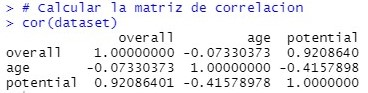
\includegraphics[scale=0.86]{./imgs/reg_correlation.jpg}
\end{figure}

El modelo elegido buscará analizar la relación de la variable (\textit{overall}) con las variables (\textit{age}) y (\textit{potential}), quedando representado de la siguiente forma:

\begin{align*}
overall = \beta_0 + potential \beta_1 + age \beta_2 + e
\end{align*}

Para investigar los resultados de la regresión y determinar el valor de los $\beta_j$ se utilizó la función "\verb|summary(regression_model)|" de \verb|R| y se obtuvo la salida mostrada en la Figura 1\\

\begin{figure}[h]
	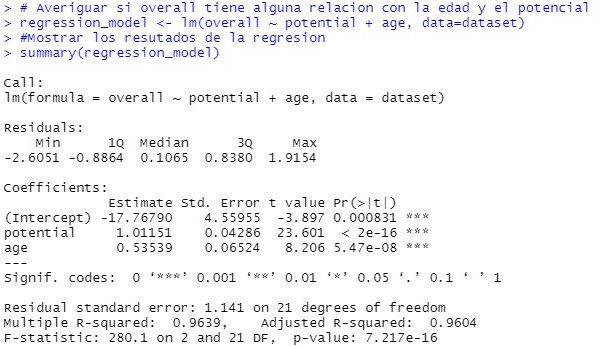
\includegraphics[scale=0.65]{./imgs/reg_model.jpg}
\end{figure}

Sustituyendo los valores obtenidos resulta el modelo:

\begin{align*}
\widehat{overall} = 1.01151 potential + 0.53539 age - 17.76790
\end{align*}

\textbf{Coeficientes}: Los coeficientes son significativos al $0\%$ inclusive el intercepto lo que es bueno para el modelo, los valores de $Pr(>|t|)$ son menores que 0.05 por lo tanto todas las variables aportan información al modelo.\\

\textbf{Adjusted R-Square}: El valor del R-Cuadrado es 0.9604 por lo tanto el modelo se considera muy bueno en cuanto a la realizaci\'on de predicciones

\textbf{F-Statistic}: Su valor menor que 0.05 nos indica la existencia de al menos una variable que esta siendo significativa para el modelo\\


\textbf{Analizando los Residuos}:

\begin{enumerate}
	\item[1.] \textbf{La media de los errores es 0 y la suma de los errores es 0}:

\begin{figure}[h]
	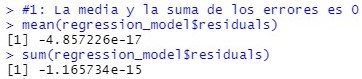
\includegraphics[scale=0.8]{./imgs/reg_1.jpg}
\end{figure}

	
	\item[2.] \textbf{Errores normalmente distribuidos}:
	Se muestra el histograma y el Normal Q-Q Plot ,en el histograma se puede apreciar un parecido a una distribuci\'on normal y al observar el QQ Plot se aprecia como la mayoría de los puntos de residuo se encuentran sobre la recta, por lo tanto se asume una normalidad en los errores del modelo (\textbf{Figura 2})
	
	\begin{figure}[h]
		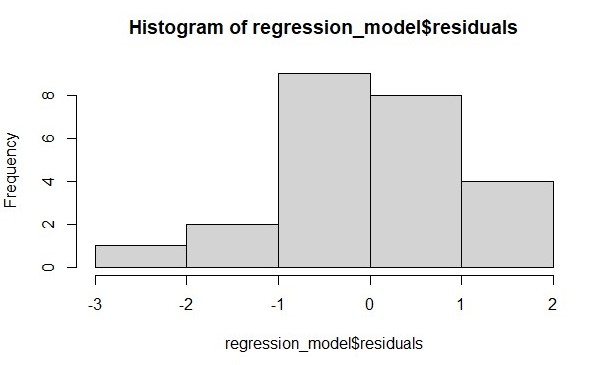
\includegraphics[scale=0.5]{./imgs/reg_2_hist.jpg}
		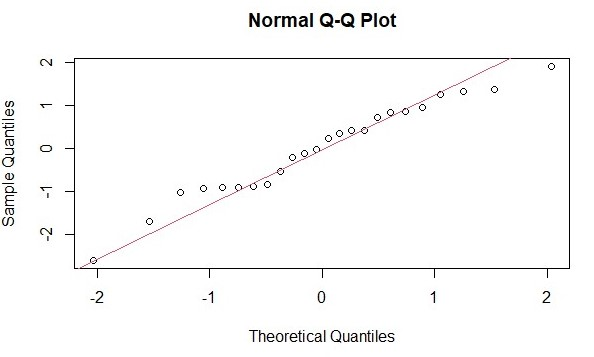
\includegraphics[scale=0.5]{./imgs/reg_2_qq.jpg}
		\caption{}
	\end{figure}
	
	\item [3.] \textbf{Independencia de los residuos}:
	Para la prueba de independencia se emplea la prueba Durbin-Watson:
	
	\begin{figure}[h]
		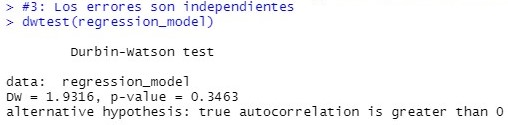
\includegraphics[width=0.5\textwidth]{./imgs/reg_3.jpg}
	\end{figure}
	
	Como el p-value es mayor que 0.05 no se puede rechazar la hipótesis nula, por lo tanto se puede afirmar que los errores son independientes. 
	
	\item[4.] \textbf{La varianza de los errores es constante (Homocedasticidad)}:
	
	Se puede observar en el gráfico el cumplimiento de la homocedasticidad:
	
	
	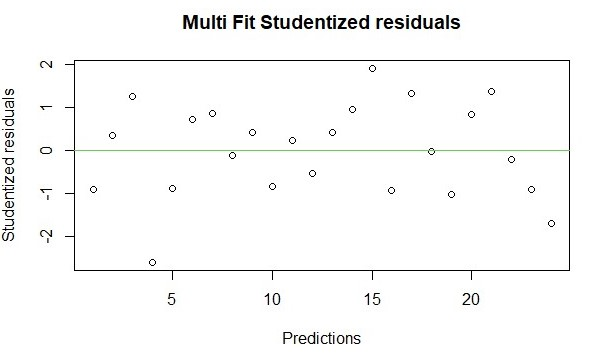
\includegraphics[scale=0.5]{./imgs/reg_4.jpg}

	
\end{enumerate}

\subsection*{ANOVA}

En este apartado se trabajará sobre el subconjunto de jugadores de campo del FIFA19 nacidos en Argentina con edades de 20, 25 y 30 años (factor edad), con el objetivo de reconocer como el físico de los jugadores varía con respecto a su edad.\\
Luego de reorganizar los datos para un correcto análisis podemos comparar las medidas de los 3 niveles del factor "edad" realizando un gráfico de cajas con las medias de cada nivel:

\begin{figure}[h]
	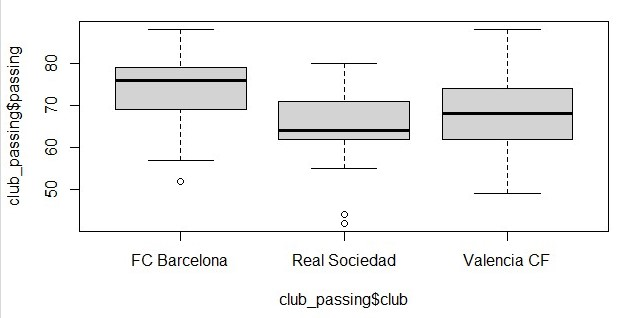
\includegraphics[scale=0.55]{./imgs/anova_boxplot.jpg}
\end{figure}

El siguiente paso sería realizar el análisis de varianza, para ver si la prueba de hipótesis es válida. En este
caso el análisis de varianza es el siguiente:

\begin{figure}[h]
	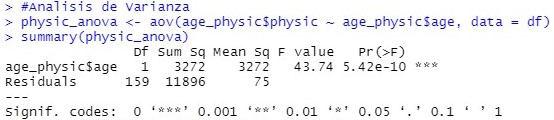
\includegraphics[scale=0.55]{./imgs/anova_summary.jpg}
\end{figure}

Como p = 0.0000 es menor que la significación prefijada $\alpha$ = 0.05, se rechaza $H_{0}$ y se acepta que al menos un grupo de futbolistas de cierta edad, tiene un físico promedio diferente. 

Por último, es necesario verificar que se cumplen los supuestos del modelo:
\begin{enumerate}
	\item Los $e_{ij}$ siguen una distribución normal con media cero.
	\item Los $e_{ij}$ son independientes entre sí.
	\item Los residuos de cada tratamiento tienen la misma varianza $\sigma^{2}$
\end{enumerate}

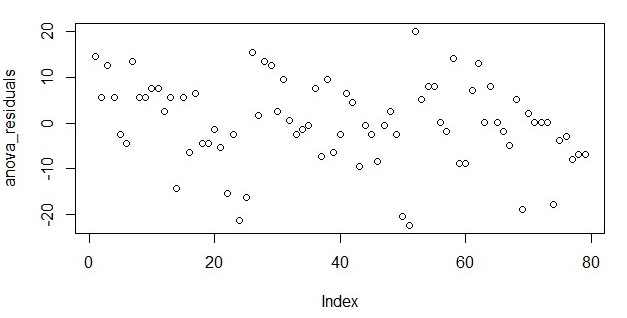
\includegraphics[scale=0.5]{./imgs/anova_residuals.jpg}
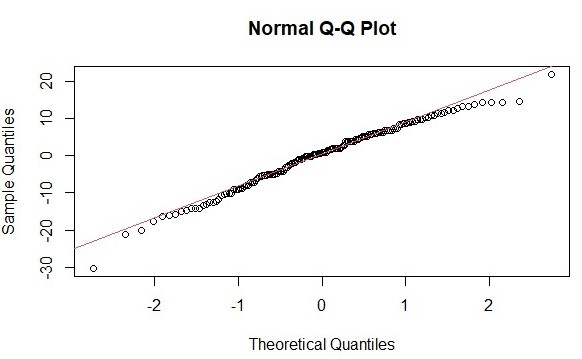
\includegraphics[scale=0.5]{./imgs/anova_qq.jpg}
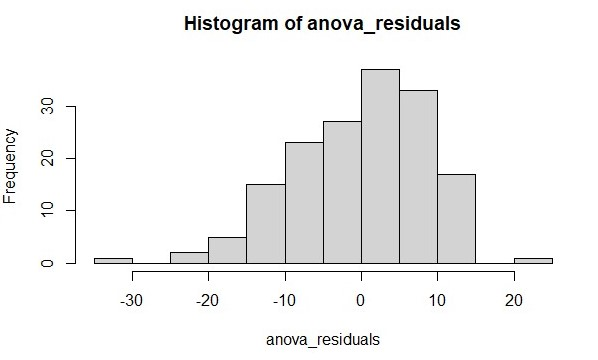
\includegraphics[scale=0.5]{./imgs/anova_hist.jpg}

Como se puede observar en el gráfico estandarizado de residuos, tienen varianza constante, el qq-plot y el histograma de residuos
muestran un comportamiento de forma normal, sin embargo, se realizarán las pruebas Shapiro-Wilcox, Bartlet y DurbinWatson para constatar el cumplimiento de los supuestos.

\begin{enumerate}
	\item Test de Shapiro-Wilcox
	
	\begin{figure}[h]
		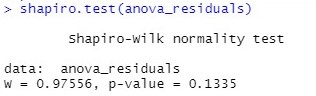
\includegraphics[scale=0.7]{./imgs/anova_shapiro.jpg}
	\end{figure}
	
	El test de Shapiro-Wilcox no es significativo (p = 0.057 $>$ 0.05), no podemos rechazar $H_{0}$ por lo que se puede confirmar la hipótesis de normalidad en los residuos.
	
	\item Test de Bartlett
	
	\begin{figure}[h]
		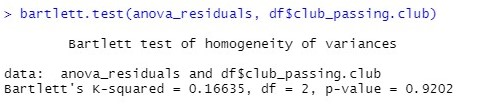
\includegraphics[scale=0.7]{./imgs/anova_bartlett.jpg}
	\end{figure}
	
	El test de Bartlett no es significativo (p = 0.97 $>$ 0.05), no podemos rechazar $H_{0}$ por lo que se puede confirmar la hipótesis de homogeneidad de las varianzas.
	
	\item Test de Durbin-Watson
	
	\begin{figure}[h]
		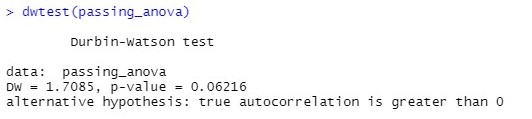
\includegraphics[scale=0.63]{./imgs/anova_dw.jpg}
	\end{figure}
	
	El test de Durbin-Watson no es significativo (p = 0.67 $>$ 0.05), no podemos rechazar $H_{0}$ por lo que se puede confirmar la hipótesis de independencia de los errores.
	
\end{enumerate}

\subsection*{ACP}

En este apartado se trabajará sobre el subconjunto de jugadores de campo del FIFA19 que pertenecen al club FC Barcelona.\\
En primera instancia se hace un análisis de la correlación en la muestra utilizando la matriz de correlación  "\verb|cor(acp_dataset)|" y la función "\verb|symnum(tp)|" presente en \verb|R|, que retorna de forma gráfica si dicha matriz esta o no, altamente correlacionada, resultando:

\begin{figure}[h]
	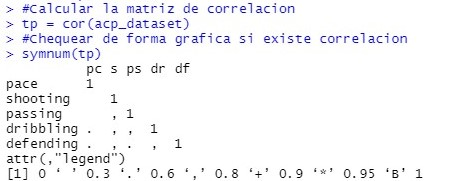
\includegraphics[scale=0.7]{./imgs/acp_correlation.jpg}
\end{figure}

Se puede observar que no existe una relación entre las variables por lo tanto se procede a reducir dimensión. Para esto se seleccionan las componentes principales:

\begin{figure}[h]
	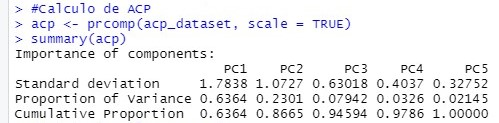
\includegraphics[scale=0.6]{./imgs/acp_summary.jpg}
\end{figure}

Para la selección de las componentes principales se emplea la proporción acumulativa, la primera componente PC1 es 0.61364 , que solo explicaría un 61\% por lo que se necesita al menos otra componente para tener un valor mayor al 70\%. Si se incluye PC2 se alcanza un 86\%. De acuerdo con el criterio de Kaiser se tiene que las dos componentes con valores propios superiores a 1 son la primera y la segunda. Por lo que PC1 y PC2 son las componentes principales a elegir. Otra forma de corroborar dicha elección sería graficar todas las componentes principales como se muestra en la siguiente gráfica:

\begin{figure}[h]
	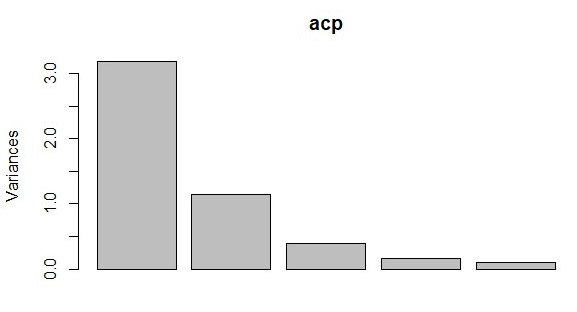
\includegraphics[scale=0.55]{./imgs/acp_plot.jpg}
\end{figure}

Para interpretar los datos se debe calcular la matriz de valores propios y así se sabrá que variable es importante para cada componente y en qué medida:

\begin{figure}[h]
	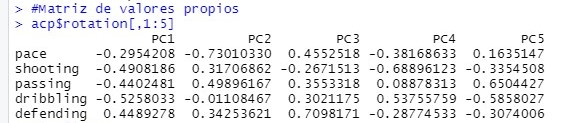
\includegraphics[width=0.5\textwidth]{./imgs/acp_vp.jpg}
\end{figure}


Para esto se analiza por cada componente el mayor valor propio $\lambda_i$, este se divide entre 2 y la variable asociada a cada valor propio cuyo valor absoluto este por encima de $\lambda_i / 2$, pertenecerá a la componente.

\begin{enumerate}
	\item[] \textbf{PC1} ($\lambda_{\max} = 0.52$): Esta componente esta caraterizada por una muestra de jugadores con estadísticas ofensivas bajas y buenas capacidades defensivas. (Defensas)
	
	\item[] \textbf{PC2} ($\lambda_{\max} = 0.73$): Esta componente esta caracterizada por una muestra de jugadores con poco ritmo pero buenos pasadores y disparando al arco. (Delantero)
	
	\item[] \textbf{PC3} ($\lambda_{\max} = 0.70$): Esta componente esta caracteriza por una muestra de	jugadores con buen ritmo, buenas capacidades defensivas y pasando el balón. (Medio Centro Defensivo) 
	
	\item[] \textbf{PC4} ($\lambda_{\max} = 0.68$): Esta componente esta caracteriza por una muestra de	jugadores con buenas habilidades en el dominio del balón, con poco ritmo y no muy finos en los disparos. (Medio Centro)
	
	\item[] \textbf{PC4} ($\lambda_{\max} = 0.65$): Esta componente esta caracteriza por una muestra de	jugadores con poca habilidad en el dominio del balón y en el disparo pero buenos pasadores. (Medio Ofensivo) 
	
\end{enumerate} 

La figura siguiente muestra un biplot para las 2 primeras componentes (PC1, PC2) con la representación de los jugadores según sus habilidades:

\begin{figure}[h]
	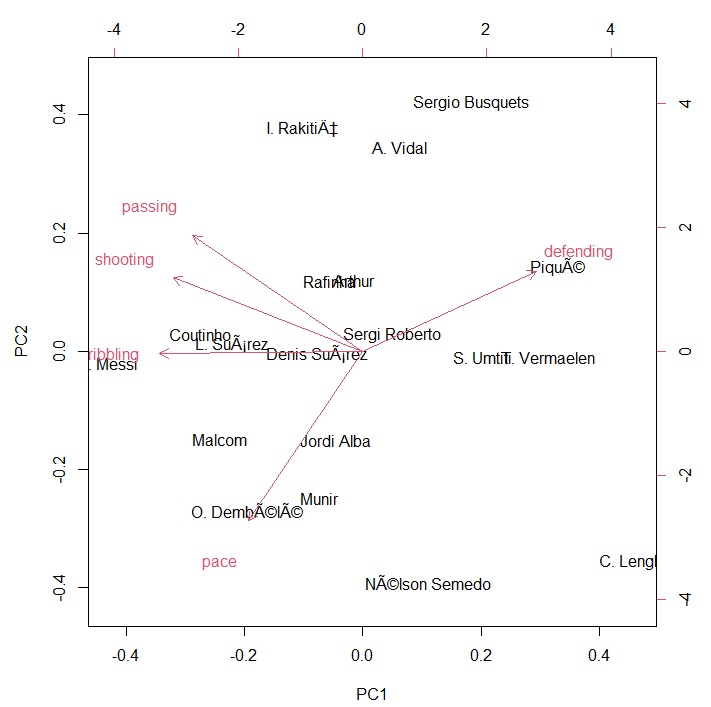
\includegraphics[scale=0.4]{./imgs/acp_biplot.png}
\end{figure}

\label{end}

\end{document}

%===================================================================================
